% Created 2024-04-11 Thu 04:12
% Intended LaTeX compiler: pdflatex
\documentclass[11pt]{article}
\usepackage[utf8]{inputenc}
\usepackage[T1]{fontenc}
\usepackage{graphicx}
\usepackage{longtable}
\usepackage{wrapfig}
\usepackage{rotating}
\usepackage[normalem]{ulem}
\usepackage{amsmath}
\usepackage{amssymb}
\usepackage{capt-of}
\usepackage{hyperref}
\usepackage[labelfont=bf]{caption}
\author{Hankertrix}
\date{\today}
\title{Machine Learning In Chemistry Literature Review}
\hypersetup{
 pdfauthor={Hankertrix},
 pdftitle={Machine Learning In Chemistry Literature Review},
 pdfkeywords={},
 pdfsubject={},
 pdfcreator={Emacs 29.3 (Org mode 9.6.15)}, 
 pdflang={English}}
\makeatletter
\newcommand{\citeprocitem}[2]{\hyper@linkstart{cite}{citeproc_bib_item_#1}#2\hyper@linkend}
\makeatother

\usepackage[notquote]{hanging}
\begin{document}

\maketitle
\setcounter{tocdepth}{2}
\tableofcontents \clearpage\newpage

\section{Abstract}
\label{sec:orgc1da452}
\(\indent\) This paper investigates the research applications of machine learning, mostly in chemistry. It will do so by looking at 3 different papers, namely "Machine Learning for Chemistry: Basics and Applications" \citeprocitem{1}{[1]}, "Rethinking drug design in the artificial intelligence era" \citeprocitem{2}{[2]}, and "The advent of generative chemistry" \citeprocitem{3}{[3]}. The applications include retrosynthesis, chemical hypothesis generation, and reducing cycle times. A brief overview of machine learning and data, as well as the issues faced with current datasets will be given, followed by a brief overview of the various applications. The difficulties and challenges faced in the various applications will be discussed, along with a brief outlook at the end. This literature review aims to show that artificial intelligence (AI) and machine learning (ML) will eventually become an important part of chemistry in the future.


\section{Introduction}
\label{sec:org9264abb}
\(\indent\) With the rise of artificial intelligence (AI) and machine learning (ML), it is important to examine their possible applications in chemistry research. AI and ML are particularly useful for tedious and repetitive tasks \citeprocitem{4}{[4]}, such as drug discovery and retrosynthesis, which are iterative processes that take a long amount of time. The current latest and greatest ML models such as ChatGPT, DALL-E 2, Midjourney and Stable Diffusion, which are all neural networks, are also generative in nature, meaning that they create things that haven't been created before \citeprocitem{5}{[5]}–\citeprocitem{7}{[7]}. This ability to generate novel items makes neural networks especially helpful in the realm of drug discovery \citeprocitem{3}{[3]}. AI and ML are also helpful in retrosynthesis, chemical hypothesis generation, and reducing cycle times.

\newpage

\section{Machine learning and data}
\label{sec:orgc4212ef}
\(\indent\) Machine learning (ML) is a branch of AI that allows computers to perform tasks without explicit instructions \citeprocitem{8}{[8]}. Most computers usually require explicit instructions in the form of code to perform their tasks \citeprocitem{9}{[9]}, \citeprocitem{10}{[10]}, but ML models "learn" to perform tasks through maths and data in a manner that is similar to biological brains \citeprocitem{11}{[11]}.
\\[0pt]

As seen in \textbf{Figure \ref{fig:orga406a12}}, the steps to train an ML model are:
\begin{enumerate}
\item Data is split into training and testing data.
\item The ML model is trained on the training data using an algorithm.
\item After the model is trained, the testing data is used to evaluate the model and improve its algorithm.
\item This cycle is repeated with new data until the model is sufficiently accurate.
\item Afterwards, the model is ready to be used.
\end{enumerate}

\begin{figure}[htbp]
\centering
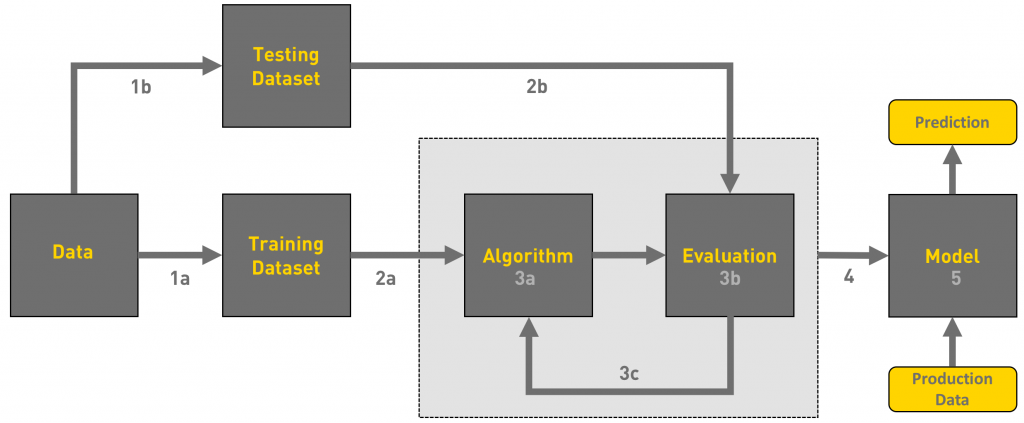
\includegraphics[width=.9\linewidth]{./images/ml-flow.png}
\caption{\label{fig:orga406a12}A flow diagram showing how an ML model learns from training data \citeprocitem{12}{[12]}.}
\end{figure}

\newpage

\subsection{Issues with data}
\label{sec:org25bd3b8}
\(\indent\) The quality of data used to train ML models greatly affects the resulting models' capability. However, data in chemistry is rarely high-quality for various reasons. Large datasets are usually designed to facilitate the testing of massive quantities of chemicals to identify their physical and chemical properties quickly. This results in the tests not being as sensitive as possible, leading to less accurate results \citeprocitem{2}{[2]}.

Another reason would be the ever-changing knowledge regarding biology, making data annotations challenging \citeprocitem{13}{[13]}, \citeprocitem{14}{[14]}. Next, misreported data can significantly impact predictive models, but ML can help identify outliers within the given dataset, pointing out potential mistakes or typos. Nevertheless, these outliers are not indicative of a mistake, only that the data point is an anomaly \citeprocitem{2}{[2]}. Also, large chemical datasets often have missing values due to time and money constraints as only the compounds suited to a high-throughput testing method will be tested, while the others will be neglected \citeprocitem{2}{[2]}. This also implies that the data is not missing at random, and hence care and consideration must be taken when using large chemical datasets \citeprocitem{2}{[2]}.

In addition, documentation of chemical experiments may be incomplete due to sheer complexity, which results in crucial variables being overlooked \citeprocitem{1}{[1]}. Furthermore, chemists rarely publish failed experiments, resulting in a lack of negative examples for ML models to learn from \citeprocitem{1}{[1]}. This bias increases the difficulty of training accurate ML models due to the reduced quantity of data and the imbalanced view of the chemical space \citeprocitem{1}{[1]}. Chemical experiments also rarely create data that can be easily translated to a single number for the ML model to process \citeprocitem{2}{[2]}, which makes model improvement difficult as most ML models are usually optimising for a single value, usually minimising something called a cost or loss function \citeprocitem{1}{[1]}. Furthermore, companies view chemical datasets as a competitive advantage, meaning that they are unwilling to share their proprietary datasets. This results in less overall data to train ML models on and results in less accurate ML models \citeprocitem{2}{[2]}. Despite this, ML has proven to be hugely useful in various chemistry applications.

\newpage

\section{Retrosynthesis}
\label{sec:org0bd460e}
\(\indent\) Retrosynthesis, also known as retrosynthetic analysis, refers to finding a synthesis pathway for a target molecule or compound by working backwards from product to reactant \textbf{(Figure \ref{fig:org78d8f5c})}. The reactants for target molecules are typically commercially available chemicals to facilitate synthesis and scalability. Neural networks are used in retrosynthesis to compute a synthetic complexity score (SCScore) to rank the molecules in retrosynthesis \citeprocitem{15}{[15]}. This hinges on the premise that reaction products are generally more synthetically complex than the reactants, meaning a larger difference between the SCScore of the products and reactants is ideal. Thus, the neural networks are trained to find synthesis pathways that have a strictly increasing SCScore. In spite of the success of ML in retrosynthesis, synthesising naturally occurring molecules remains a challenge due to the lack of data on complex molecules. Most ML models also do not consider the yield of enantiomers, which results in improper evaluation of synthesis pathways \citeprocitem{1}{[1]}.

\begin{figure}[htbp]
\centering
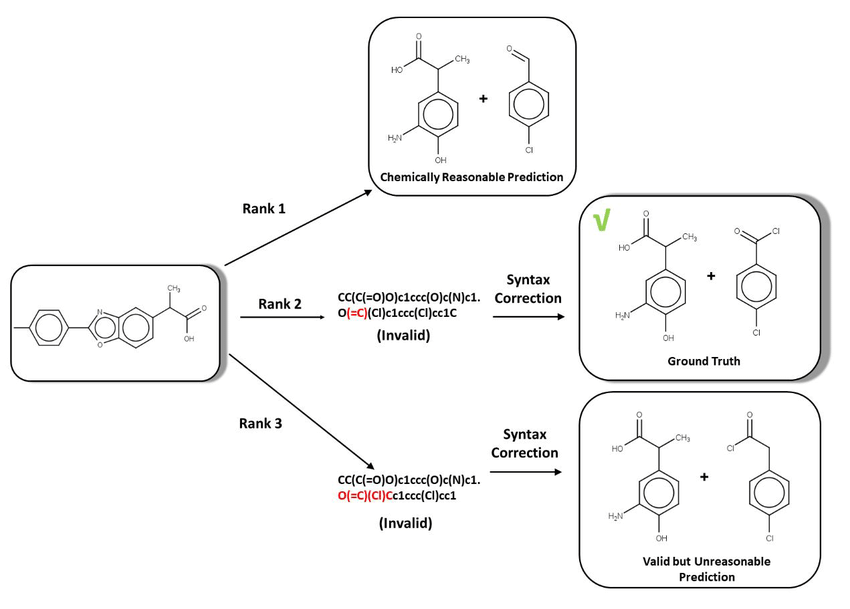
\includegraphics[width=.9\linewidth]{./images/retrosynthesis.png}
\caption{\label{fig:org78d8f5c}A diagram showing an example of retrosynthesis \citeprocitem{16}{[16]}. The target molecule is the molecule on the left side of the image, while the reactants that are found are on the right side of the image.}
\end{figure}


\section{Chemical hypothesis generation}
\label{sec:org6823437}
\(\indent\) Chemical hypothesis generation is basically the generation of molecules or chemicals that have a set of properties and functions \citeprocitem{2}{[2]}, \citeprocitem{17}{[17]}. The set of properties and functions that the chemical should have is called the hypothesis \citeprocitem{17}{[17]}. There are a lot of different ML models that have been used in chemical hypothesis generation such as recurrent neural networks (RNNs), variational autoencoders (VAEs), adversarial encoders (AAEs), and generative adversarial networks (GANs) \citeprocitem{2}{[2]}, \citeprocitem{3}{[3]}. Most of these ML models are first trained on massive datasets to learn the grammar for the simplified molecular-input line-entry system (SMILES) \textbf{(Figure \ref{fig:orgd1e17b8})} and are later refined by being trained on datasets containing molecules that have the desired properties and functions described in the hypothesis \citeprocitem{3}{[3]}.

\begin{figure}[htbp]
\centering
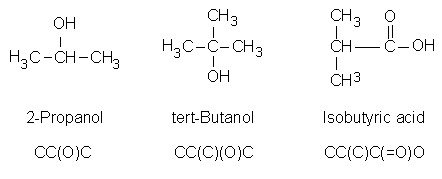
\includegraphics[width=.9\linewidth]{./images/smiles-ex-1.jpg}
\caption{\label{fig:orgd1e17b8}An example of the simplified molecular-input line-entry system (SMILES) representation, which is at the bottom \citeprocitem{18}{[18]}. SMILES is a way to represent the structure of molecules with only text.}
\end{figure}

\newpage

\subsection{Examples}
\label{sec:orgb769275}
\(\indent\) One example of such a model is an RNN based on the long short-term memory (LSTM) architecture \textbf{(Figure \ref{fig:org60b280c})}. The LSTM model enables RNNs to store and retain information longer by using memory, with the forget gate deciding on retention, the input gate determining the value of an input, and the output gate as the final model output \textbf{(Figure \ref{fig:org60b280c})}. This model was trained on the SMILES-encoded ChEMBL database, and was then fine-tuned using compounds that were active against 2 receptors \citeprocitem{19}{[19]}. Specifically, retinoid X receptors (RXRs) and peroxisome proliferator-activated receptors (PPARs) \citeprocitem{19}{[19]}. The ML model will thus generate novel compounds that are active against these 2 receptors due to this fine-tuning \citeprocitem{3}{[3]}.

\begin{figure}[htbp]
\centering
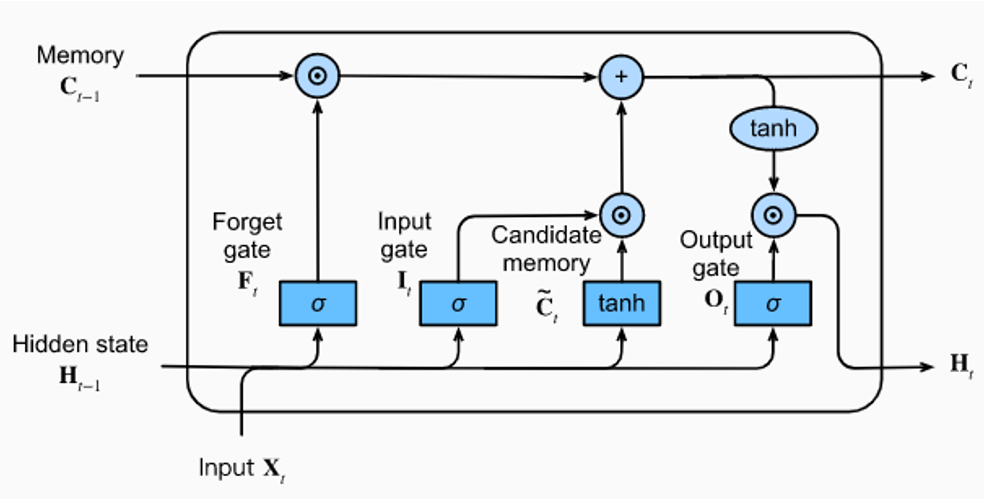
\includegraphics[width=.9\linewidth]{./images/lstm-model.png}
\caption{\label{fig:org60b280c}A diagram showing the LSTM architecture \citeprocitem{20}{[20]}.}
\end{figure}

\newpage

Another example is a VAE model trained on the SMILES representation of publicly available chemical structures in the ZINC and QM9 databases \citeprocitem{21}{[21]}. This model encoded molecules in a continuous representation, which allows the model to create molecules by stepping through the continuous graph, like in a normal distribution \citeprocitem{3}{[3]} \textbf{(Figure \ref{fig:orgff36cd6})}. The VAE decoder then converted this continuous representation back into molecular representations \citeprocitem{3}{[3]}. This continuous representation resulted in generated molecules which were optimal, due to their desired drug-like properties \citeprocitem{3}{[3]}.

\begin{figure}[htbp]
\centering
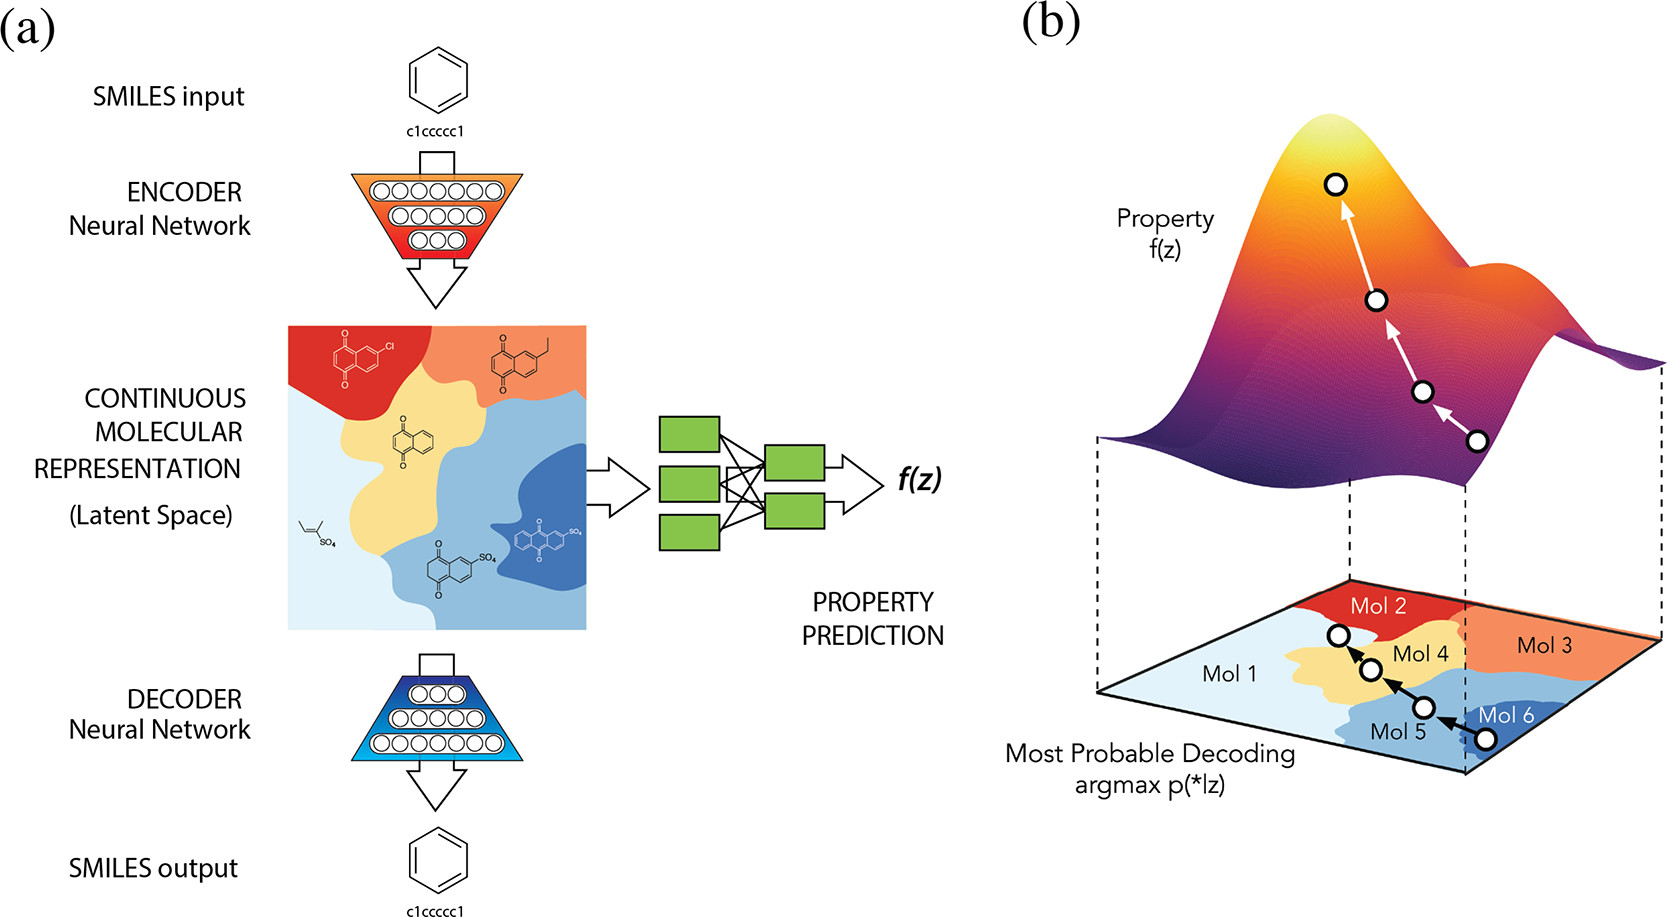
\includegraphics[width=.9\linewidth]{./images/vae-model.jpeg}
\caption{\label{fig:orgff36cd6}(a) A diagram of the VAE. (b) A diagram showing the continuous representation of molecules.}
\end{figure}

\newpage

\subsection{Reinforcement learning (RL)}
\label{sec:orge9dcb8d}
\(\indent\) Reinforcement learning (RL) \citeprocitem{22}{[22]} is often used to fine-tune these generative models by rewarding and punishing the models. This makes the models more effective in generating chemical hypotheses as they are more likely to produce compounds with the desired properties. An example of RL being applied to GANs is the objective-reinforced generative adversarial network (ORGAN) \citeprocitem{23}{[23]}. The model adds reward functions for related objectives, which are particular chemical sequences or fragments in this case \citeprocitem{23}{[23]} \textbf{(Figure \ref{fig:orge134cef})}. This causes the ML model to favour the molecules that contain these particular chemical sequences or fragments, resulting in more desired molecules being generated.

\begin{figure}[htbp]
\centering
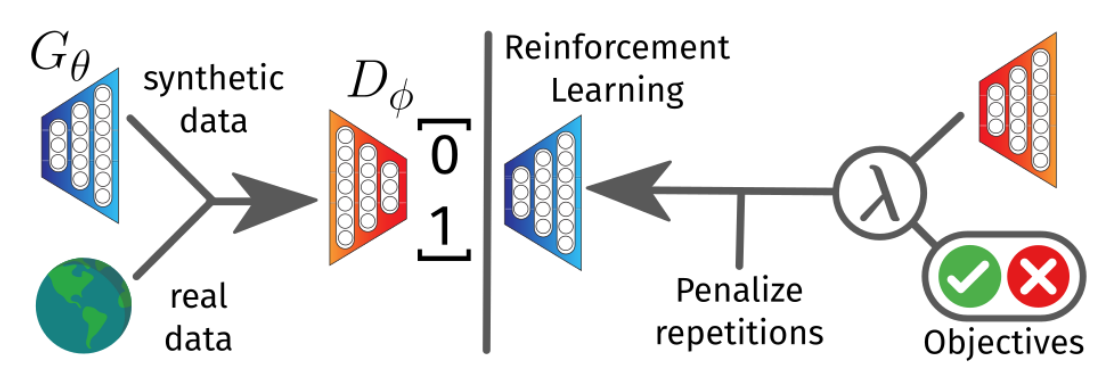
\includegraphics[width=.9\linewidth]{./images/organ-schema.png}
\caption{\label{fig:orge134cef}Schema for ORGAN. On the left, D is trained on a mix of generated data by G, and real data, to become a classifier. On the right, G is trained by RL where the reward is a combination of D and the objectives. The sequences that are not unique are punished \citeprocitem{23}{[23]}.}
\end{figure}

\newpage

\subsection{Problems}
\label{sec:orgae4ffbe}
\(\indent\) However, despite the promising results of initial AI-based generative models, there are still limitations. SMILES representation used by these models cannot incorporate reward functions favouring particular chemical sequences or fragments, as the SMILES representation makes it impossible to find chemical fragments \citeprocitem{3}{[3]}. One solution is to use other ways of representing molecules, such as graph representations, which are basically the skeletal formula of a molecule. Additionally, evaluating generative AI models can be challenging due to insufficient documentation regarding their capabilities \citeprocitem{3}{[3]}.

In addition, the effects of drugs on the biological systems do not always map well to the chemical structure of a drug, and the effects are usually muddied up by multiple confounding factors that are usually unknown \citeprocitem{3}{[3]}. As a result, the behaviour of the AI model is ultimately unpredictable as the structure of a drug doesn't necessarily correspond to its function \citeprocitem{3}{[3]}. This additional complexity is not always taken into account, which makes molecular scoring a complex task \citeprocitem{3}{[3]}. Current molecular scoring functions are also not very appropriate, resulting in a more difficult fine-tuning and optimisation of drugs for desired properties \citeprocitem{3}{[3]}.

Furthermore, generated molecules are usually difficult to synthesise, which greatly limits the practical use of such molecules. Even though the molecules are AI-generated, there is still a lot of manual input required to make the generated molecules easier to synthesise \citeprocitem{3}{[3]}. This is usually the case when the chemicals required are unavailable, unstable, insufficiently reactive or require lengthy preparation. However, it is a problem that can be solved by using ML in retrosynthesis to find easier synthesis pathways for the generated molecules.

\newpage

\section{Reducing cycle times}
\label{sec:org5c1c48b}
\(\indent\) There is considerable investment of time and money in the discovery of new drugs, and the risk of failure at all stages of the drug discovery process is high \citeprocitem{2}{[2]}. Thus, it would be ideal to use ML models to automate the process of new drug discovery. Currently, profiling capabilities have been improving, but the massive increase in the number of data points makes it onerous for the human brain to keep up \citeprocitem{2}{[2]}. This results in scientists using simple heuristics and efficiency metrics \citeprocitem{24}{[24]}–\citeprocitem{26}{[26]} which are less than ideal \citeprocitem{27}{[27]}, but it has not resulted in any improvement in the cycle times needed to create new drugs \citeprocitem{2}{[2]}.

\begin{figure}[htbp]
\centering
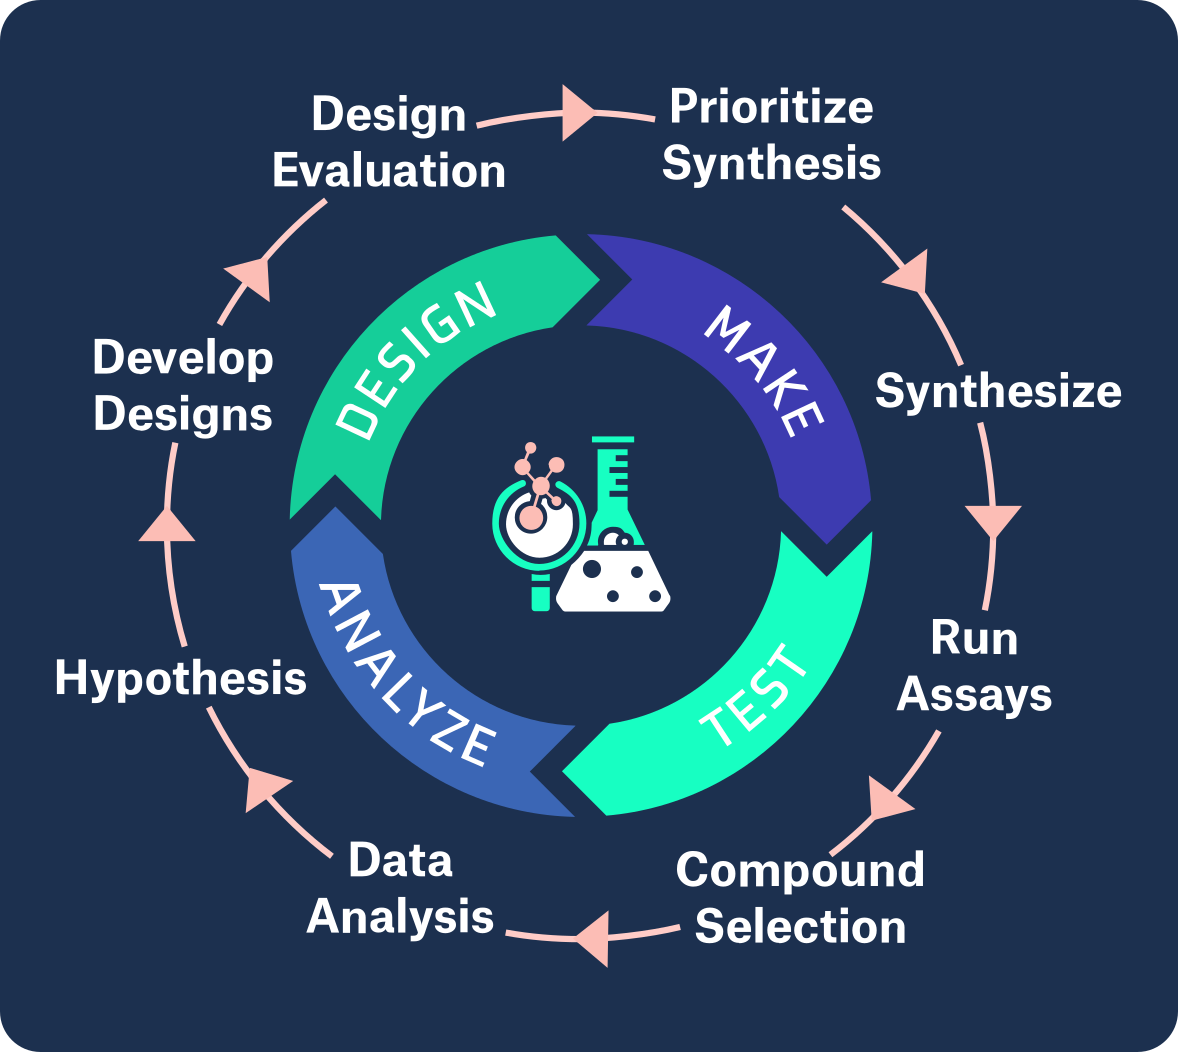
\includegraphics[height=22em]{./images/dmta-cycle.png}
\caption{\label{fig:org376252c}An illustration of the design-make-test-analyse (DMTA) cycle \citeprocitem{28}{[28]}.}
\end{figure}

The main process in drug discovery is the design-make-test-analyse (DMTA) cycle \textbf{(Figure \ref{fig:org376252c})} \citeprocitem{29}{[29]}. Available data is first used to generate hypotheses and design compounds. The designed compounds are then synthesised and tested to figure out if the hypotheses are correct. The knowledge gained from one DMTA cycle is then put into the development of design hypotheses for the next DMTA cycle \citeprocitem{2}{[2]}. Automating this DMTA cycle would have a sizeable impact on drug discovery \citeprocitem{29}{[29]}, \citeprocitem{30}{[30]}.
\\[0pt]

The benefits of automation include \citeprocitem{31}{[31]}:
\begin{itemize}
\item Reduced measurement errors and material consumption as computers excel in accuracy, unlike humans.
\item Faster feedback loops for AI-Based hypothesis generation and optimisation.
\item Opportunities to increase the number of ways to synthesise compounds, like microfluidic-assisted synthesis and reactions under extreme conditions \citeprocitem{32}{[32]}.
\item Prioritising compounds that are effective in humans using cellular testing of the compounds \citeprocitem{33}{[33]}–\citeprocitem{35}{[35]}.
\item Optimisation without any personal bias.
\end{itemize}

Automated DMTA platforms have already shown their efficiency in drug design and optimisation in the reduced amount of time it takes to complete a DMTA cycle \citeprocitem{36}{[36]}. In the case of the researchers at AbbVie, they could obtain results within 1 - 2 days \citeprocitem{37}{[37]}.

However, DMTA cycles still take a long time, often taking more than 4 - 8 weeks to complete \citeprocitem{2}{[2]}. The slow "make" phase of the cycle, responsible for synthesising new molecules, can take several weeks \citeprocitem{2}{[2]}. Consequently, shortening this phase is crucial for reducing DMTA cycle times. To expedite the process, laboratory automation with automatic analytics and purification is key \citeprocitem{31}{[31]}, \citeprocitem{32}{[32]}, \citeprocitem{38}{[38]}, \citeprocitem{39}{[39]}.

To maximise efficiency, multiple DMTA cycles are often performed simultaneously, and the cycles are often left incomplete \citeprocitem{2}{[2]}. This ensures that the chemicals are synthesised before all the data is available, effectively addressing design hypotheses \citeprocitem{40}{[40]}. However, the accumulation of data becomes challenging to record and analyse, \citeprocitem{2}{[2]}. To cope with this difficulty, scientists often rely on rules of thumb \citeprocitem{41}{[41]}, efficiency metrics, model systems like logP or logD, or matched molecular pairs \citeprocitem{42}{[42]} to make sense of the data. Searching for trends, insights and patterns is intellectually taxing and runs the risk of being overwhelming, resulting in important conclusions being missed.

\newpage

Thus, there is potential for AI to enhance DMTA cycles by assisting chemists with molecule design hypotheses and data analysis \citeprocitem{43}{[43]}. AI could also look for improved synthesis routes and optimise reaction conditions so that the synthesis of molecules is done correctly the first time, shortening the "make" phase \citeprocitem{44}{[44]}–\citeprocitem{47}{[47]}. It can also provide timely and context-specific recommendations to researchers \citeprocitem{48}{[48]}, reducing the time spent reviewing raw data \citeprocitem{2}{[2]}. However, this requires a documented data trail, standardised concepts to describe the data, and access to raw data when needed \citeprocitem{2}{[2]}.

\section{Future outlook}
\label{sec:org8639ebe}
\(\indent\) The current spotlight on ML suggests that ML applications in research will continue to improve. Companies are now seriously considering ML to automate workflows and reduce errors when they might not have before. The surge in popularity of AI and ML is likely to attract a lot of young talents to the field of ML, particularly computer science graduates. These talents could bring a fresh perspective and may eventually come up with novel ways of applying ML to chemistry. With an increasingly automated world, AI robots may soon conduct experiments and analyse data, automating the DMTA cycle and allowing researchers to focus on fine-tuning the generated molecules. Such automation could result in standardised documentation and benchmarks to maximise efficiency. ML and automation may lead to faster DMTA cycles as laboratory procedures and experiments may be increasingly designed with them in mind. This will eventually make AI and ML a crucial part of chemistry in the future when most laboratory processes are automated and AI and ML-based tools are being used to automate chemical discovery.

\newpage

\section{References}
\label{sec:orgd4f2a09}
\(\indent\) Below is the list of references used in this literature review:
\\[0pt]

\hypertarget{citeproc_bib_item_1}{[1] Y.-F. Shi \textit{et al.}, “Machine learning for chemistry: Basics and applications,” \textit{Engineering}, 2023.}

\hypertarget{citeproc_bib_item_2}{[2] P. Schneider \textit{et al.}, “Rethinking drug design in the artificial intelligence era,” \textit{Nature reviews drug discovery}, vol. 19, no. 5, pp. 353–364, 2020.}

\hypertarget{citeproc_bib_item_3}{[3] Q. Vanhaelen, Y.-C. Lin, and A. Zhavoronkov, “The advent of generative chemistry,” \textit{Acs medicinal chemistry letters}, vol. 11, no. 8, pp. 1496–1505, 2020.}

\hypertarget{citeproc_bib_item_4}{[4] T. H. Davenport, \textit{The ai advantage: How to put the artificial intelligence revolution to work}. mit Press, 2018.}

\hypertarget{citeproc_bib_item_5}{[5] A. Borji, “Generated faces in the wild: Quantitative comparison of stable diffusion, midjourney and dall-e 2,” \textit{Arxiv preprint arxiv:2210.00586}, 2022.}

\hypertarget{citeproc_bib_item_6}{[6] K. Roose, “An ai-generated picture won an art prize. artists aren’t happy,” \textit{The new york times}, vol. 2, no. September, 2022.}

\hypertarget{citeproc_bib_item_7}{[7] R. Gozalo-Brizuela and E. C. Garrido-Merchan, “Chatgpt is not all you need. a state of the art review of large generative ai models,” \textit{Arxiv preprint arxiv:2301.04655}, 2023.}

\hypertarget{citeproc_bib_item_8}{[8] D. Bzdok, M. Krzywinski, and N. Altman, “Machine learning: a primer,” \textit{Nature methods}, vol. 14, no. 12, p. 1119, 2017.}

\hypertarget{citeproc_bib_item_9}{[9] B. W. Kernighan and D. M. Ritchie, “The c programming language,” 2002.}

\hypertarget{citeproc_bib_item_10}{[10] D. A. Rusling, “The linux kernel.” 1999.}

\hypertarget{citeproc_bib_item_11}{[11] E. Alpaydin, \textit{Introduction to machine learning}. MIT press, 2020.}

\hypertarget{citeproc_bib_item_12}{[12] A. Pant, “Workflow of a machine learning project,” \textit{Medium}. Towards Data Science, Jan. 2019. Available: \url{https://towardsdatascience.com/workflow-of-a-machine-learning-project-ec1dba419b94?gi=3390a5f49b26}}

\hypertarget{citeproc_bib_item_13}{[13] Y. Lin \textit{et al.}, “Drug target ontology to classify and integrate drug discovery data,” \textit{Journal of biomedical semantics}, vol. 8, pp. 1–16, 2017.}

\hypertarget{citeproc_bib_item_14}{[14] R. Santos \textit{et al.}, “A comprehensive map of molecular drug targets,” \textit{Nature reviews drug discovery}, vol. 16, no. 1, pp. 19–34, 2017.}

\hypertarget{citeproc_bib_item_15}{[15] C. W. Coley, L. Rogers, W. H. Green, and K. F. Jensen, “Scscore: synthetic complexity learned from a reaction corpus,” \textit{Journal of chemical information and modeling}, vol. 58, no. 2, pp. 252–261, 2018.}

\hypertarget{citeproc_bib_item_16}{[16] S. Zheng, J. Rao, Z. Zhang, J. Xu, and Y. Yang, “Predicting retrosynthetic reactions using self-corrected transformer neural networks,” \textit{Journal of chemical information and modeling}, vol. 60, no. 1, pp. 47–55, 2019.}

\hypertarget{citeproc_bib_item_17}{[17] P. W. Sprague, “Automated chemical hypothesis generation and database searching with catalyst,” \textit{Perspectives in drug discovery and design}, vol. 3, no. 1, pp. 1–20, 1995.}

\hypertarget{citeproc_bib_item_18}{[18] Imperius, “Smile always, it is smiles notation!,” \textit{Smile always, it is smiles notation!} Nov. 2013. Available: \url{https://imperius1234.blogspot.com/2013/11/smile-always-it-is-smiles-notation.html}}

\hypertarget{citeproc_bib_item_19}{[19] D. Merk, L. Friedrich, F. Grisoni, and G. Schneider, “De novo design of bioactive small molecules by artificial intelligence,” \textit{Molecular informatics}, vol. 37, no. 1-2, p. 1700153, 2018.}

\hypertarget{citeproc_bib_item_20}{[20] O. Calzone, “An intuitive explanation of lstm,” \textit{Medium}. Medium, Apr. 2022. Available: \url{https://medium.com/@ottaviocalzone/an-intuitive-explanation-of-lstm-a035eb6ab42c}}

\hypertarget{citeproc_bib_item_21}{[21] R. Gómez-Bombarelli \textit{et al.}, “Automatic chemical design using a data-driven continuous representation of molecules,” \textit{Acs central science}, vol. 4, no. 2, pp. 268–276, 2018.}

\hypertarget{citeproc_bib_item_22}{[22] K. Arulkumaran, M. P. Deisenroth, M. Brundage, and A. A. Bharath, “A brief survey of deep reinforcement learning,” \textit{Arxiv preprint arxiv:1708.05866}, 2017.}

\hypertarget{citeproc_bib_item_23}{[23] G. L. Guimaraes, B. Sanchez-Lengeling, C. Outeiral, P. L. C. Farias, and A. Aspuru-Guzik, “Objective-reinforced generative adversarial networks (organ) for sequence generation models,” \textit{Arxiv preprint arxiv:1705.10843}, 2017.}

\hypertarget{citeproc_bib_item_24}{[24] N. A. Meanwell, “Improving drug design: an update on recent applications of efficiency metrics, strategies for replacing problematic elements, and compounds in nontraditional drug space,” \textit{Chemical research in toxicology}, vol. 29, no. 4, pp. 564–616, 2016.}

\hypertarget{citeproc_bib_item_25}{[25] M. M. Cavalluzzi, G. F. Mangiatordi, O. Nicolotti, and G. Lentini, “Ligand efficiency metrics in drug discovery: The pros and cons from a practical perspective,” \textit{Expert opinion on drug discovery}, vol. 12, no. 11, pp. 1087–1104, 2017.}

\hypertarget{citeproc_bib_item_26}{[26] A. L. Hopkins, G. M. Keserü, P. D. Leeson, D. C. Rees, and C. H. Reynolds, “The role of ligand efficiency metrics in drug discovery,” \textit{Nature reviews drug discovery}, vol. 13, no. 2, pp. 105–121, 2014.}

\hypertarget{citeproc_bib_item_27}{[27] P. W. Kenny, A. Leitao, and C. A. Montanari, “Ligand efficiency metrics considered harmful,” \textit{Journal of computer-aided molecular design}, vol. 28, pp. 699–710, 2014.}

\hypertarget{citeproc_bib_item_28}{[28] Strateos, “Automating the dmta cycle for small molecules,” \textit{Strateos}. Mar. 2022. Available: \url{https://strateos.com/automated-dmta/}}

\hypertarget{citeproc_bib_item_29}{[29] A. T. Plowright, C. Johnstone, J. Kihlberg, J. Pettersson, G. Robb, and R. A. Thompson, “Hypothesis driven drug design: improving quality and effectiveness of the design-make-test-analyse cycle,” \textit{Drug discovery today}, vol. 17, no. 1-2, pp. 56–62, 2012.}

\hypertarget{citeproc_bib_item_30}{[30] D. M. Parry, “Closing the loop: developing an integrated design, make, and test platform for discovery,” \textit{Acs medicinal chemistry letters}, vol. 10, no. 6, pp. 848–856, 2019.}

\hypertarget{citeproc_bib_item_31}{[31] M. Nettekoven and A. W. Thomas, “Accelerating drug discovery by integrative implementation of laboratory automation in the work flow,” \textit{Current medicinal chemistry}, vol. 9, no. 23, pp. 2179–2190, 2002.}

\hypertarget{citeproc_bib_item_32}{[32] T. Dimitrov, C. Kreisbeck, J. S. Becker, A. Aspuru-Guzik, and S. K. Saikin, “Autonomous molecular design: then and now,” \textit{Acs applied materials \& interfaces}, vol. 11, no. 28, pp. 24825–24836, 2019.}

\hypertarget{citeproc_bib_item_33}{[33] L. H. Jones and M. E. Bunnage, “Applications of chemogenomic library screening in drug discovery,” \textit{Nature reviews drug discovery}, vol. 16, no. 4, pp. 285–296, 2017.}

\hypertarget{citeproc_bib_item_34}{[34] R. M. Eglen and D. H. Randle, “Drug discovery goes three-dimensional: goodbye to flat high-throughput screening?,” \textit{Assay and drug development technologies}, vol. 13, no. 5, pp. 262–265, 2015.}

\hypertarget{citeproc_bib_item_35}{[35] E. W. Esch, A. Bahinski, and D. Huh, “Organs-on-chips at the frontiers of drug discovery,” \textit{Nature reviews drug discovery}, vol. 14, no. 4, pp. 248–260, 2015.}

\hypertarget{citeproc_bib_item_36}{[36] M. Trobe and M. D. Burke, “The molecular industrial revolution: automated synthesis of small molecules,” \textit{Angewandte chemie international edition}, vol. 57, no. 16, pp. 4192–4214, 2018.}

\hypertarget{citeproc_bib_item_37}{[37] A. Vasudevan, A. Bogdan, H. Koolman, Y. Wang, and S. Djuric, “Enabling chemistry technologies and parallel synthesis—accelerators of drug discovery programmes,” \textit{Progress in medicinal chemistry}, vol. 56, pp. 1–35, 2017.}

\hypertarget{citeproc_bib_item_38}{[38] J. A. Selekman \textit{et al.}, “High-throughput automation in chemical process development,” \textit{Annual review of chemical and biomolecular engineering}, vol. 8, pp. 525–547, 2017.}

\hypertarget{citeproc_bib_item_39}{[39] R. D. King \textit{et al.}, “Make way for robot scientists,” \textit{Science}, vol. 325, no. 5943, p. 945, 2009.}

\hypertarget{citeproc_bib_item_40}{[40] M. D. Segall, “Multi-parameter optimization: identifying high quality compounds with a balance of properties,” \textit{Current pharmaceutical design}, vol. 18, no. 9, p. 1292, 2012.}

\hypertarget{citeproc_bib_item_41}{[41] J. S. Scott and M. J. Waring, “Practical application of ligand efficiency metrics in lead optimisation,” \textit{Bioorganic \& medicinal chemistry}, vol. 26, no. 11, pp. 3006–3015, 2018.}

\hypertarget{citeproc_bib_item_42}{[42] E. Griffen, A. G. Leach, G. R. Robb, and D. J. Warner, “Matched molecular pairs as a medicinal chemistry tool: miniperspective,” \textit{Journal of medicinal chemistry}, vol. 54, no. 22, pp. 7739–7750, 2011.}

\hypertarget{citeproc_bib_item_43}{[43] G. Hessler and K.-H. Baringhaus, “Artificial intelligence in drug design,” \textit{Molecules}, vol. 23, no. 10, p. 2520, 2018.}

\hypertarget{citeproc_bib_item_44}{[44] A.-C. Bédard \textit{et al.}, “Reconfigurable system for automated optimization of diverse chemical reactions,” \textit{Science}, vol. 361, no. 6408, pp. 1220–1225, 2018.}

\hypertarget{citeproc_bib_item_45}{[45] C. W. Coley, W. H. Green, and K. F. Jensen, “Machine learning in computer-aided synthesis planning,” \textit{Accounts of chemical research}, vol. 51, no. 5, pp. 1281–1289, 2018.}

\hypertarget{citeproc_bib_item_46}{[46] M. H. Segler, M. Preuss, and M. P. Waller, “Planning chemical syntheses with deep neural networks and symbolic ai,” \textit{Nature}, vol. 555, no. 7698, pp. 604–610, 2018.}

\hypertarget{citeproc_bib_item_47}{[47] S. Szymkuć \textit{et al.}, “Computer-assisted synthetic planning: the end of the beginning,” \textit{Angewandte chemie international edition}, vol. 55, no. 20, pp. 5904–5937, 2016.}

\hypertarget{citeproc_bib_item_48}{[48] S. L. Rohall, M. Pancost-Heidebrecht, B. Shirley, D. Bacon, and M. A. Tarselli, “Recommendations for chemists: a case study,” in \textit{Proceedings of the 12th acm conference on recommender systems}, 2018, pp. 347–351.}\bigskip

\[\text{Word count: } 2189\]
\end{document}
